\chapter{Search Engine}
Die Twitter-Klon Applikation soll mit einer Suchfunktion erweitert werden. Diese Suchfunktion wird mit einem Such-Service umgesetzt, der auf der Elasticsearch-Engine basiert. Elasticsearch setzt auf Apache Lucene auf, einer in Java geschriebenen Bibliothek für die Volltextsuche. Es ist open-source, dokumentenorientiert, in Java geschrieben und lässt sich über einen REST-API ansprechen. Damit ist es ein guter Kandidat für unser Use-Case.

\section{Zielsetzung}
Das Ziel des Suchservices ist die Ausgabe von \textit{best-match} Ranglisten über eine Tweets-Sammlung zu erstellen, indem man nach bestimmten Benutzern, Tags und Freitexteingaben sucht. Als Erweiterung der Suchfunktion wird ein Text-Vervollständigung Feature erstellt, das beim Suchen nach Tweets passende Vorschläge liefert. Und zum Schluss sollen ausgewählte Datensätze, mit Hilfe eines Analyse- und Visualisierungstools, auf der Homepage als eine Grafik angezeigt werden. 

\section{Vorgehen}
Zuerst wird eine \textit{Elasticsearch-Service} Architektur angefertigt. Diese stellt nur ein Teil der \textit{Twitter-Klon} Umsetzung und behandelt die Kommunikation zwischen \textit{Elasticsearch}, \textit{Elasticsearch-Service} wie den \textit{Kafka-Topics}. Nachfolgend wird Elasticsearch entsprechend der \textit{Twitter-Klone} Applikation konfiguriert und für die Datenaufnahmen vorbereitet. Infolgedessen wird der Such-Service implementiert, der \textit{Elasticsearch} mit den \textit{Kafka-Topics} verbindet und für den Datenaustausch zuständig ist. Anschließend werden Datenvisualisierungen mit Hilfe von \textit{Kibana} angefertigt. Zum Schluss wird der Elasticsearch Abschnitt mit einem Fazit beendet.

\section{Service Design}
Der komplette Nachrichtenaustauch der \textit{Twitter-Klon} Applikation wird mit einem skalierbaren und performanten Messaging-Service umgesetzt, nämlich \textit{Apache Kafka}. Dieser, bietet die Möglichkeit, mit Hilfe der Nachrichten-Topics den Overhead an Kommunikation zwischen den Services zu verringern, die Services von einander zu entkoppeln und die Daten parallel zu verarbeiten.
Diese Eigenschaft ermöglicht das Entkoppeln des Such-Service‘es von dem Restsystem, sodass die Suche unabhängig von den Schnittstellen der heterogenen Klienten bedient werden kann. 
Dafür wurden drei Topics erstellt und ein Datenformat vereinbart, das langfristig alle unsere Wünsche abdecken soll. Die Such-Service Use-Cases sind in drei Gruppen eingeteilt, die mit Hilfe von drei Kafka-Topics realisiert wurden: Neue Dokumente indexieren/abspeichern, Anfragen empfangen und Anfragen beantworten.
%\captionsetup{justification = raggedright,singlelinecheck = false}
\begin{figure}[htbp!]
  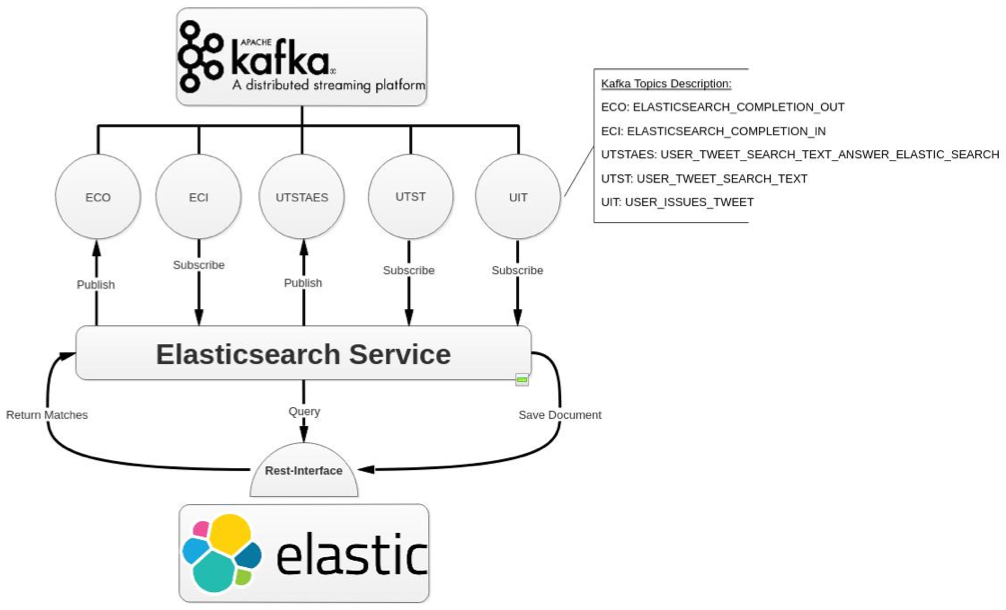
\includegraphics[scale=0.8]{material/architecture/Elasticsearch.png}
  \caption{Elasticsearch Service Architectur}
  \label{fig:ESA}
\end{figure}

Der Such-Service meldet sich an den entsprechenden Kafka-Topics an, öffnet ein Datenstrom und empfängt Nachrichten mit den Speicher-, Suchkriterien, sowie der dazugehörigen Benutzerkennung. Um den Speicherplatz optimal zu nutzen, werden aus der Nachricht nur für die Suche relevante Felder ausgelesen und an die Elasticsearch REST-Schnittstelle weitergeleitet, wie z.B. der Text, die Benutzerkennung, die Tags und der Zeitstempel.  

Das Verschicken der Nachrichten über unsere Applikation durchläuft den \textit{UIT} Topic, dieser bietet jedem Abonnenten den Zugriff auf die neu eingetroffenen Mitteilungen. Der Elasticsearch-Suchservice ist einer der bestehenden Abonnenten des \textit{UIT} Topics und bereitet die neu eingetroffenen Nachrichten für die Weiterleitung und das Speichern des Inhalts in Elasticsearch. Die, mit Metainformation bestückten, Nachrichten laufen eine Transformation durch wie Filterung, Umbenennung und Umstrukturierung, um der Elasticsearch erwarteten Datenstruktur zu entsprechen und Speicherplatz zu sparen. 

Für die Suchfunktion werden die Topics \textit{UTST} und \textit{UTSTAES} genutzt. Über den \textit{UTST} werden Suchanfragen entgegengenommen und in eine Elasticsearch-Rest-Anfrage umgeformt. Die Suchanfrage kann von dem Suchservice auf verschiedene Weise durchgeführt werden. Zum Beispiel durch eine Term-, Bollean-, Match-, Multimatch- und Match-Phrase- Suche. Jede Abfrageart, kann im bestimmten Fällen vorteilhaft ausgenutzt werden und kann Fallspezifisch eingesetzt werden. 
Das Suchergebnis wird anschließend als eine sortierte Identifikationsliste zu enthaltenen Nachrichten auf dem \textit{UTSTAES} Topic hinterlegt. Damit wäre die Suche beendet und das weitere Geschehen des Suchergebnisses den \textit{UTSTAES} Abonnenten überlassen.

Die Suchvervollständigung verhält sich ähnlich der Suchfunktion. Der Suchservice kommuniziert über die Topics \textit{ECI} und \textit{ECO}, die vervollständigung Anfragen für die Benutzereingabe publizieren und mögliche Eingabewünsche entgegennehmen. Die Eingabewünsche könne mit Hilfe der Elasticsearch Vervollständigung oder durch die nGrams-Implementation umgesetzt werden. Diese Ansätze sind in der Granularität, Umsetzung, Laufzeit und Speicherbedarf unterschiedlich und könne Fallabhängig ausgetauscht werden. 


\section{Elasticsearch Konfiguration}
Elasticsearch funktioniert \textit{out of the box}, das heißt, man muss den Service nur starten und das Indexieren, wie das Suchen der Dokumente funktioniert reibungslos. Im Gegensatz zu den relationalen Datenbanken ist eine Schema Definition für Elasticsearch nicht notwendig. Obwohl ein Schema nicht gefordert ist, ist es höchst ratsam dieses zu deferieren, denn das \textit{Type-Matching} der Felder wird ansonsten nach dem \textit{Best Guess} Prinzip erstellt und kann unter umstanden zum unerwünschten Verhalten führen.

\subsection{Index Settings}
Die \textit{out of the box} Fähigkeit von Elasticsearch ist toll zum Ausprobieren, jedoch ist es für den Betrieb ungeeignet, da die Einstellungen für die bestmögliche Skalierung von Elasticsearch, wie das Durchsuchen der Texte immer von der Domäne abhängt. Falsche oder keine Anpassung, kann die Skalierungsmöglichkeiten von Elasticsearch drastisch senken und damit den Betrieb unerwartet unterbrechen. Des Weiteren ist die Anpassung der Textvorverarbeitung eine Kernaufgabe jeder Such-Engine, dementsprechend sollte man sich besonders sorgfältig um diese Aufgabe kümmern, sodass alle relevanten Ergebnisse ermittelt und in einer passenden Ordnung dem Nutzer vorgelegt werden können.

\subsection{Sharding \& Replication}
Zuerst wird der Elasticsearch Index auf Shards und Replicas aufgeteilt. Damit enthält ein Shard eine Teilinformation oder ein Replikat der Teilinformation des Indexes, der auf unterschiedliche Hardware aufgeteilt werden kann. Obwohl die Verschiebung des Shards Knotenübergreifend realisiert werden kann, kann dieser nicht in zwei neue Shards gespalten werden, wenn die Hardware an ihre Grenzen stößt. Damit ist ein Shard die Skalierungseinheit des Indexes und muss sorgfältig gewählt werden. Der uns gegebene Elasticsearch Cluster arbeitet nur auf einem Knoten, dementsprechend ist der Skalierungsfaktor von fünf genug um zukunftssicher den Index bis auf fünf weitere Knoten aufteilen zu können. Der Replikationsfaktor beschreibt wie viele Replikate für einen Shard erstellt werden. Für eine Einstellung aus fünf Shards und einem Replikat entsteht eine Gesamtdatenmenge von 10 Shards. Daraus folgt ein immenser Anstieg an Speicherverbrauch für jeden nächsten Replikat eines Shardes. Die Replikate bieten im Gegensatz die Ausfallsicherheit und die Performance Steigerung der Lesezugriffe. Da die Performance und die Ausfallsicherheit für jeder skalierbare Applikation Kernkriterien sind, kann Elasticsearch diese bei Bedarf im laufenden Betrieb durch neue Replikate stärken. In unserem Fall steht nur einen Knoten zur Verfügung, dementsprechend folgt kein Anstieg der Performance wie Ausfallsicherheit mit Hilfe der Replikation.
% Bild  mit Reploikation der Shards und Replikas auf Knoten.
\\\\
\textbf{Initiale Index Einstellungen}
\begin{lstlisting}[language=json,firstnumber=1]
{
  "twitterindex": {
    "settings": {
      "index": {
        "number_of_shards": "2",
        "number_of_replicas": "0",
        "refresh_interval": "1s",
        "provided_name": "twitterindex",
        "creation_date": "1529674155106",
        ...
        "uuid": "wOHQnu5GQjOs7iP-Cv-_MQ",
        "version": {
          "created": "6020399"
        }
      }
    }
  }
}
\end{lstlisting}

\subsection{Textvorverarbeitung}
Als nächstes wird der Textvorverarbeitungsprozess definiert. Unter dem Schlüssel \textit{Analyzer} wird ein \textit{Custom Analyzer} und die dazugehörigen Vorverarbeitungsschritte erstellt. Dieser wird innerhalb Elasticsearch aufbewahrt und mit Funktionalität belegt. Der Analyzer zerlegt den Text mit dem \textit{Partial Word Tokenizer} in Tokens nach einem bestimmten Muster, nämlich nach einem Leerzeichen, nach einem Großbuchstaben Anfang und nach einer Zahl.
Dieser Zerlegungsschritt erfüllt die gegebenen Anforderungen, könnte aber auf Kosten des Speicherplatzes durch den mächtigeren \textit{Edge NGram Tokenizer} ausgetauscht werden. Nachfolgend laufen die Tokens eine Transformationskette durch. Zuerst werden die Tokens in Kleinbuchstaben umgewandelt, auf den Wortstamm zurückgeführt und Worte mit geringen Informationsgehalt, sowie verboten Worte entfernt. Zuletzt werden die Worte mit ähnlicher Bedeutung wie \textit{Universität Hamburg} und \textit{UHH} in Synonymlisten zusammengefasst und als gleichgültig behandelt. 
\\\\
\textbf{Analyzer}
\begin{lstlisting}[language=json,firstnumber=1]
"analyzer": {
...
  "my_analyzer": {
    "filter": [
      "my_tokenizer",
      "lowercase",
      "my_stemmer",
      "english_possessive_stemmer",
      "my_stop",
      "my_synonym"
    ],
    "type": "custom",
    "tokenizer": "standard"
  },
...
}
\end{lstlisting}

\subsection{Data Mapping}
Zuletzt braucht Elasticsearch ein Datenschema, um die automatische Fehleinschätzung des Mappings zu vermeiden. 
Elasticsearch baut einen Suchindex auf, der Dokumentenbasiert in einem JSON Format abgespeichert wird. Das Mapping garantiert eine Typenzusicherung wie das Format, der zu speichernden Felder und Dokumente. Zum Beispiel das Datumformat, das Regionsunabhängig vor dem Abspeichern von Elasticsearch normalisiert wird oder das Textfeld, das man mit bestimmten Eigenschaften und Funktionen anreichert, um das gewünschte Verhalten zu realisieren. 
Der Text, kann als \textit{Keyword} abgespeichert werden, das Eins-zu-eins durchsucht wird oder ein \textit{Text}, das mit Hilfe der Volltextsuche komplexen Suchkriterien umsetzen kann.
Das Elasticsearch Mapping für den Twitter-Klon definiert ein Dokumentenformat mit sieben Felder: id, message, tags, users, timeStamp, userLocation und userLocationCompletion. Für die Suche sind die Felder \textit{message}, \textit{tags} und \textit{use} relevant, diese werden vom Type \textit{Keyword} und \textit{Text} gespeichert. Das Feld \textit{timeStamp} wird auf ein \textit{Long} projiziert und für die Datenvisualisierung mit Kibana genutzt, um die wöchentlichen Trends anzuzeigen. Das Feld \textit{userLocation} hält die vom Benutzer eingetragene Standort, der mit der Textvervollständigungsinformation von Elasticsearch angereichert und durch das Feld \textit{userLocationCompletion} beschrieben. Zum Vergleich wird das Feld \textit{userLocation}  zusätzlich mit dem \textit{nGram Analyzer} belegt, um die Text-Verfollständigung von Elasticsearch mit der \textit{nGram} Methode vergleichen zu können.  
\\\\
\textbf{Mapping}
\begin{lstlisting}[language=json,firstnumber=1]
"userLocation": {
  "type": "text",
  "analyzer": "nGram_analyzer",
  "search_analyzer": "nGram_search_analyzer"
},
"userLocationCompletion": {
  "type": "completion",
  "analyzer": "simple",
  "preserve_separators": true,
  "preserve_position_increments": true,
  "max_input_length": 50
},
\end{lstlisting}


\section{Search Service}
Die Implementation des Such Service wird mit Java und Spring realisiert. Spring ist ein weit verbreitetes und etabliertes Enterprise Framework für Java. Dieses besitz eine große Palette an Werkzeigen, die das Arbeiten in einer heterogenen Umgebung stark vereinfachen. Daher eignet sich Spring besonders gut für unseren Anwendungsfall. Für den Nachrichtenaustausch zwischen Apache Kafka, Elasticsearch und dem Suchservice wird, die von Spring entwickelte \textit{Spring for Apache Kafka} und die von Elasticsearch angebotene \textit{Elasticsaerch Rest Client} Bibliotheken genutzt.
Die interne Logik des Suchservices wird von den Java Beans umgesetzt, die im Springkontext auf dem Apache Tomcat Application Server ausgeführt werden und die gewünschte Such-Funktionalität umsetzen.

\subsection{Such-Interface}
Um die Kommunikation und Fähigkeiten des Such Services übersichtlich zu gestalten, wird ein Interface mit den gewünschten Anfragen erstellt und anschließend implementiert. 

\begin{enumerate}
  \item über die Tags
  \item über die referenzierten Benutzer
  \item über angegebenen Standortnamen mit der Textvervollständigung
  \item über die Term-Suche auf den Tweet-Text
  \item über die Volltextsuche auf den Tweet-Text
  \item über den Text wie den Benutzet Standortnamen
  \item über einen Zeitraum
  \item über einen Zeitraum mit Benutzer und Tag Präferenz 
\end{enumerate}

\subsection{Such-Implementation}
Elasticsearch bietet eine JSON-ähnliche domänenspezifische Sprache, mit der man Abfragen ausführen kann. Dies wird als \textit{DSL Query} bezeichnet. Die Abfragesprache ist ziemlich umfassend und bietet komplexe Filter und Aggregation Möglichkeiten. Die Anfragen des Suchservices sind ausgelegt die wichtigsten Anfragemöglichkeiten von Elasticsearch darzustellen. Es werden \textit{term}, \textit{match}, \textit{multi match}, \textit{match phrase}, \textit{bool}, \textit{compleation} und \textit{aggregation} Anfragen behandelt. 
\\\\
\textbf{Suchen nach Tags}
\begin{lstlisting}[language=json,firstnumber=1]
{
  "query": {
    "terms": {
      "tags.keyword": "?"
         }
    }
}
\end{lstlisting}

\textbf{Suche nach Referenzierten Benutzer}
\begin{lstlisting}[language=json,firstnumber=1]
{
  "query": {
    "terms": {
      "users.keyword": "?"
    }
  }
}
\end{lstlisting}

Die Tag- und Benutzersuche wird mit der Term-Suche umgesetzt, diese sucht nach Dokumenten, die genau, die im angegebenen Feld angegebenen Begriffe enthalten. Die Tweets werden entsprechend den TF/IDF Relevanz sortiert und präsentiert.  
\\\\
\textbf{Textvervollständigung nach Standortnamen}
\begin{lstlisting}[language=json,firstnumber=1]
{
  "suggest": {
    "location_suggest": {
      "prefix": "?",
      "completion": {
        "field": "userLocationCompletion",
        "fuzzy": {
          "fuzziness": 1
        }
      }
    }
  }
}
\end{lstlisting}
Der Textvervollständigung bietet Funktionen zur automatischen Vervollständigung. Es werden Vorschläge wehrend des Tippens einer Anfrage getätigt und führt schneller zu relevanten Ergebnissen. Durch die zusätzliche \textit{fuzzy} Eigenschaft der Abfrage werden zusätzlich Tippfehler abgefangen um die Suche den Nutzer angenehmer zu gestalten.
\\\\
\textbf{Term-Suche auf den Tweet-Text}
\begin{lstlisting}[language=json,firstnumber=1]
{
  "query": {
    "match": {
      "message": "?"
    }
  }
}
\end{lstlisting}

\textbf{Volltextsuche auf den Tweet-Text}
\begin{lstlisting}[language=json,firstnumber=1]
{
  "query": {
    "match_phrase": {
      "message": {
        "query": "?",
        "slop": 1
      }
    }
  }
}
\end{lstlisting}

Die Suche über den Textkörper eines Tweets kann auf zwei Arten getan werden. Im ersten Fall wird eine Match-Suche \textit{metch} durchgeführt, diese normalisiert die Suchterme, verknüpft sie mit \textit{OR} und durchsucht den Textkörper nach Suchbegriff-Treffern. Im zweiten Fall nutzt man die zusammenhängende Suchanfrage \textit{phrase match}, welche im Gegensatz zu \textit{match} die Terme mit \textit{AND} verknüpft und eine Einschränkungen mitbringt, nämlich die Ordnung der Suchterme im Textkörper. Um die Suche flexibler zu gestalten, kann sie aufgeweicht werden, indem man die akzeptable Entfernung der Suchterme mit der \textit{Slope} Eingeschalt beeinflusst. In unseren Fall erlaubt diese eine Entfernung von einem Wort zwischen den Suchbegriffen.

\textbf{Standortabhängige Tweets}
 \begin{lstlisting}[language=json,firstnumber=1]
 {
  "query": {
    "multi_match": {
      "query": "?",
      "fields": [
        "message",
        "userLocation"
      ]
    }
  }
}
\end{lstlisting}

Die \textit{multi match} Abfrage sucht nach Nachrichten, dessen Inhalt einen Ort verweist und der Autor sich in dieser Region befindet. Diese Abfrage verhält sich wie \textit{match}, jedoch über eine Menge von Feldern.
\\\\
\textbf{Suche Tweets über den Zeitraum mit referenzierte Benutzer zuerst}
 \begin{lstlisting}[language=json,firstnumber=1]
{
  "query": {
    "bool": {
      "must": {
        "terms": {
          "tags": "?"
        }
      },
      "filter": {
        "range": {
          "timeStamp": {
            "gte": "now-1d/d",
            "lt": "now/d"
          }
        }
      },
      "should": [
        {
          "term": {
            "users": "?"
          }
        }
      ]
    }
  }
}
\end{lstlisting}
Diese Suchanfrage führt ein neues Konzept der \textit{bool} Anfrage, die aus mehreren Komponenten besteht. Die Suche besteht aus erforderlichen Feld-Treffern wie den optionalen Feld-Treffern. Daraus ergibt sich eine Rangordnung aus den relevanten Ergebnissen. Zuletzt läuft die Liste einen Zeitfilter durch um den Zeitraum einzuschränken. 
\\\\
\textbf{Top Tweets für die letzten sieben Tage }
 \begin{lstlisting}[language=json,firstnumber=1]
{
  "aggs": {
    "top_tags": {
      "significant_terms": {
        "field": "tags",
        "size": 10
      }
    }
  },
  "query": {
    "bool": {
      "must": [
        {
          "match_all": {}
        },
        {
          "range": {
            "timeStamp": {
              "gte": "now-7d/d",
              "lt": "now/d"
            }
          }
        }
      ]
    }
  }
}
\end{lstlisting}
Diese Anfrage ist zuständig für die Visualisierung in Kibana. In diesem Fall wird mit Hilfe der \textit{bool} Anfrage und der Elasticsearch-Aggregation, die am häufigsten verwendeten Tag über den Datensatz von sieben Tagen erarbeitet.  
\\\\
\section{Visualisierung mit Kibana}
Die Visualisierungsmöglichkeiten von Kibana sollen es ermöglichen große Datenmengen zu analysieren unterstützt durch flexible Filter. Es bietet Echtzeit-Analyse von Daten, individuell konfigurierbare Visualisierung, dynamische Dashboards und Browserbasiertes Interface, das Plattformunabhängige funktioniert.\\\\
Die Kibana Visualisierungen basieren auf den Aggregationsmöglichkeiten von Elasticsearch. Dieses aggregiert über den Elasticsearch Indexinhalt und erstellt Grafiken, die in HTML eingebunden werden können. Zur Verfügung stehende Visualisierungstypen: Area Chart, Data Table, Line Chart, Markdown Widget, Mertric, Pie Chart, Tile Map, Vertical Bar Chart.
%\captionsetup{justification = raggedright,singlelinecheck = false}
\begin{figure}[htbp!]
  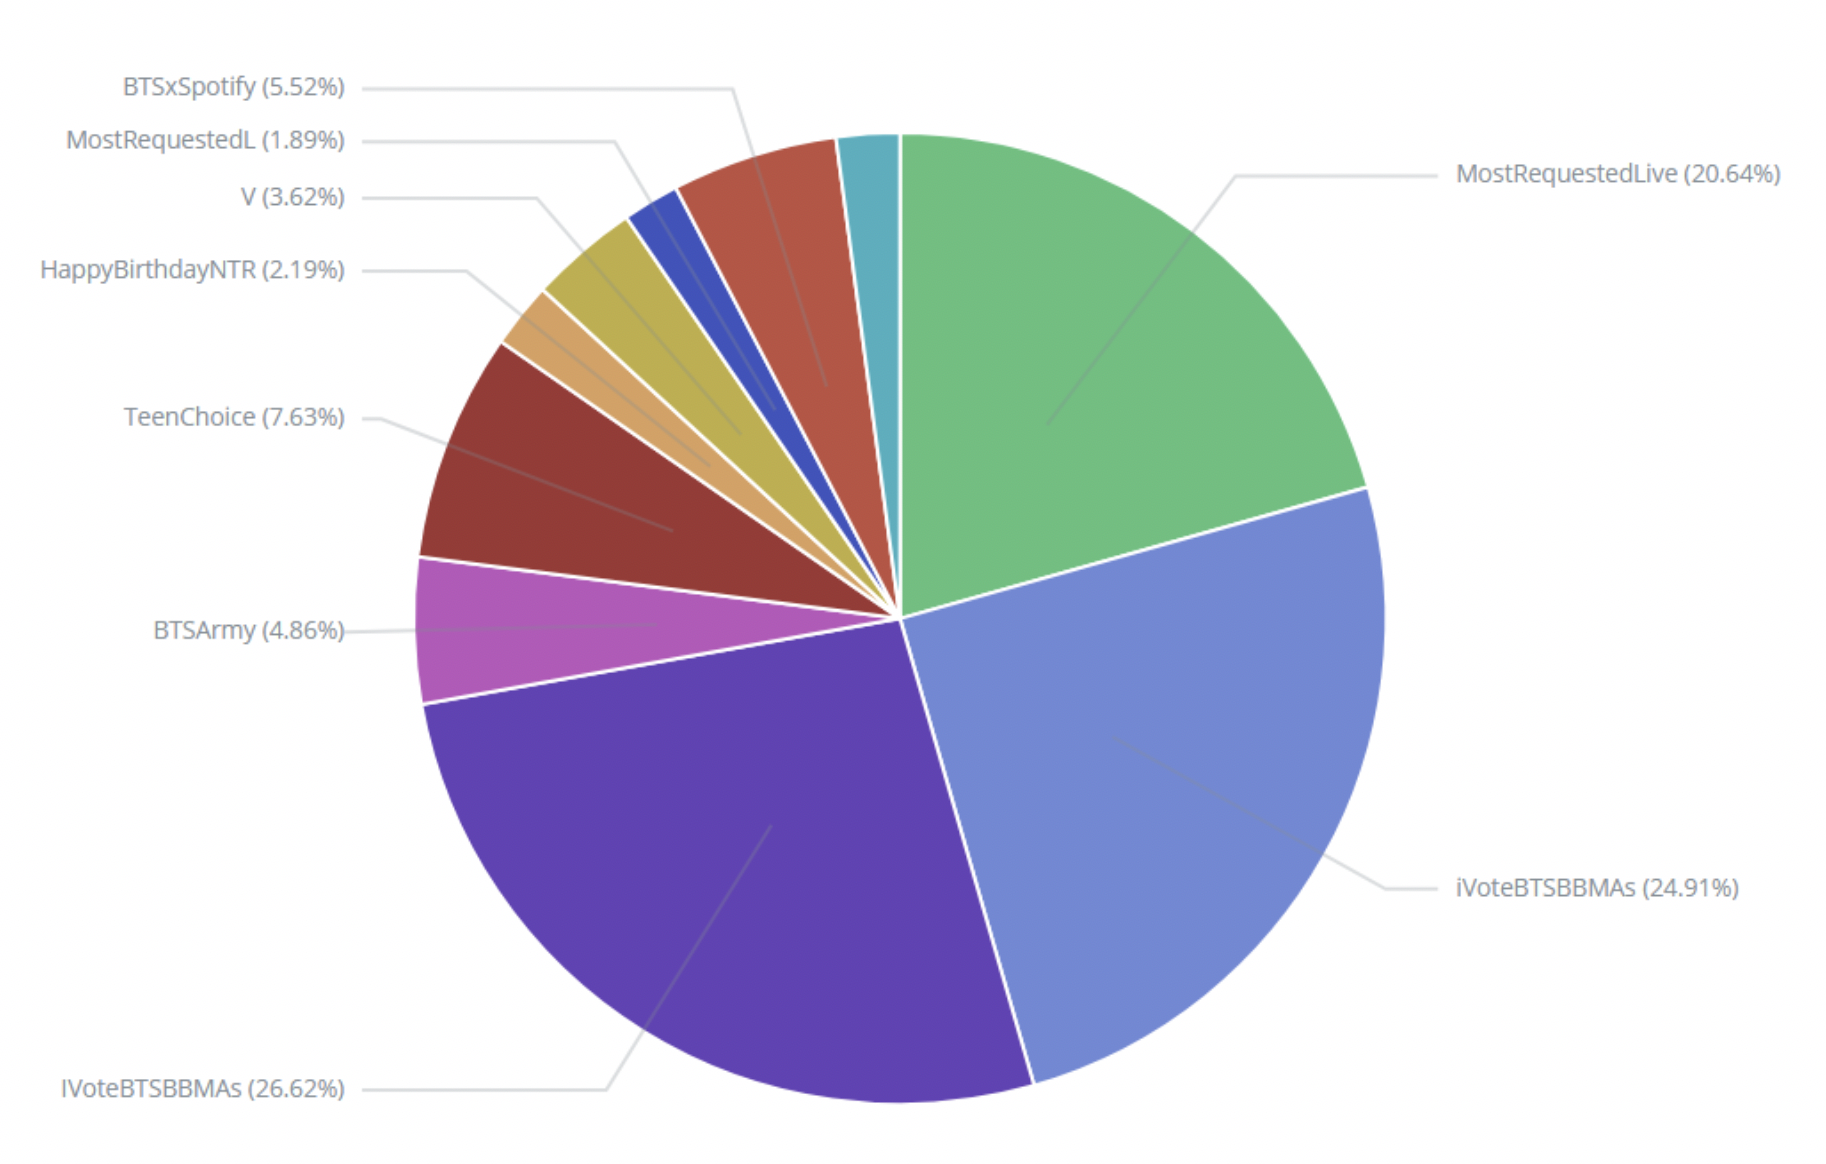
\includegraphics[scale=0.4]{material/architecture/kibana.png}
  \caption{Kibana Analyseplattform} 
  \label{fig:Kibana}
\end{figure}

\section{Fazit}
\subsection{Suchfunktionalität}
Jede moderne Software bietet eine Möglichkeit nach Daten zu suchen. Mit Hilfe von Elasticsearch kann eine einfache Suche nach einer Website oder einem Dokument innerhalb einer Sammlung implementiert werden. Anschließend kann eine Rechtschreibprüfung hinzugefügt werden. Höchstwahrscheinlich ist eine fuzzy Suche und automatische Vervollständigung nötig, möglicherweise sogar während der Eingabe. Da die Relevanz wichtig ist, können fortgeschrittene Ranking-Schemata erstellt werden. Zum Beispiel können Suchergebnisse basierend auf dem Standort, Zeit sowie des Benutzers ausgeführt werden. Und um zu wissen, was die Benutzer tatsächlich tun, kann die Nutzung der Software protokolliert und gespeichert werden für die spätere Analyse der Nutzerdaten.
\newline
Damit ist Elasticsearch eine moderne und mächtige Such-Engine, die fortgeschrittene Suchfunktionalität anbietet und für viele Anwendungsfälle geeignet ist.

\subsection{Performance}
Elasticsearch hat sich als eine robuste und fähige Such-Engine bewiesen, es konnte alle Ziele ohne Einschränkungen erfüllen und zusätzlich mit einer Vervollständigungsfunktion ergänzen. Die Index Konfiguration lässt sich einfach bedienen und über kleine Kalibrierungsschritte im JSON Format von einfachen bist komplexen Indexstrukturen erstellen. Von den Shards, Replicas bis zu den Data-Routings ist Cluster übergreifend alles möglich. Das Suchen ist eine etablierte IT-Disziplin, die mit Komfort, Kosten und Gewinn fest verbunden ist. Demgemäß ist Elasticsearch perfekt geeignet große Datenmengen zu durchsuchen und scheint mit der Anfragegeschwindigkeit, die mit jedem weiteren gefüllten Hardwareknoten die Anfragen automatisch parallelisiert. 
Somit bleibt die Geschwindigkeit im grünen Bereich auch nach dem Anstieg der Datenmenge.  
Allerdings haben die positiv gelisteten Eigenschaften ihre Tücken. Die Konfiguration des Indexes kann im Kleien so wie im Großen geschehen. Die richtige Hardware- (RAM/SSD/HDD) wie Indexkonfiguration muss gewissenhaft gewählt werden, um die versprochenen Geschwindigkeiten zu erreichen. Dementsprechend gewinnt man Zeit durch die automatisierte Datenverwaltung und verliert durch die Elasticsearch Wartung/Feinabstimmung. 

\subsection{Dokumentation und API}
Ebenso problematisch sind die Elasticsearch Abfragen, die einerseits gut im JSON-Format beschrieben und dokumentiert sind, jedoch in der Umsetzung, durch die von Elasticsearch zur Verfügung gestellten JAVA Bibliothek in JAVA schwer verständlich und Komplex in der Umsetzung.
Erst zum Ende des Projekts bin ich auf \textit{Mustach} gestoßen, die \textit{JSON-Templats} für die Abfragen erstellt und diese in einer simplen Form an Elasticsearch weiterleitet.  

\subsection{Tools} 
Besondere positiv aufgefallen ist die WebUI Kibana die mit Elasticsearch über REST Anfragen kommuniziert. Es ist möglich nach Daten zu suchen, den Clusterstatus abzufragen sowie aussagekräftige Grafiken zu erstellen. Diese Werkzeuge bieten dem Entwickler einen einfachen und übersichtlichen Einstig in die Elasticsearch-Umgebung.    
